\documentclass[conference]{IEEEtran}
\IEEEoverridecommandlockouts
\usepackage{cite}
\usepackage{amsmath,amssymb,amsfonts}
\usepackage{algorithmic}
\usepackage{graphicx}
\usepackage{textcomp}
\usepackage{enumitem}
\usepackage{xcolor}
\usepackage{booktabs}
\usepackage{multirow}
\usepackage{tikz}
\usetikzlibrary{arrows.meta,positioning,fit,calc,shapes.geometric,backgrounds}
\usepackage[caption=false,font=footnotesize]{subfig}
\usepackage{pgfplots}
\pgfplotsset{compat=1.18}
\tikzset{
  pipbox/.style={draw,rounded corners=2pt,align=center,inner sep=3pt,minimum height=0.72cm,font=\footnotesize},
  pipsmall/.style={draw,rounded corners=2pt,align=center,inner sep=2pt,font=\footnotesize,minimum height=0.60cm},
  arr/.style={-Latex,thick,shorten >=1pt,shorten <=1pt},
  arrd/.style={-Latex,thick,dashed,shorten >=1pt,shorten <=1pt}
}
\def\BibTeX{{\rm B\kern-.05em{\sc i\kern-.025em b}\kern-.08em
    T\kern-.1667em\lower.7ex\hbox{E}\kern-.125emX}}

\graphicspath{{./}{figures/}}

\begin{document}

\title{Noise-Aware Pipeline for Indian Bird Sound Classification\\
Using BirdNET Embeddings, Focal-Loss MLP, and Autoencoder Gating}

\author{%
\IEEEauthorblockN{Samarth D Kolur}
\IEEEauthorblockA{\textit{Computer Science and Technology}\\
\textit{Dayananda Sagar University}\\
Bengaluru, India\\
samarthdkolur1@gmail.com}
\and
\IEEEauthorblockN{Yashaswini R}
\IEEEauthorblockA{\textit{Computer Science and Technology}\\
\textit{Dayananda Sagar University}\\
Bengaluru, India\\
rygowda1703@gmail.com}
\and
\IEEEauthorblockN{Mithun Krishnan}
\IEEEauthorblockA{\textit{Computer Science and Technology}\\
\textit{Dayananda Sagar University}\\
Bengaluru, India\\
mithunkrishnan82@gmail.com}
\and
\IEEEauthorblockN{Manoj C}
\IEEEauthorblockA{\textit{Computer Science and Technology}\\
\textit{Dayananda Sagar University}\\
Bengaluru, India\\
manojchandrashekhar.058@gmail.com}
\and
\IEEEauthorblockN{Dr.\ Ramandeep Kaur}
\IEEEauthorblockA{\textit{Computer Science and Technology}\\
\textit{Dayananda Sagar University}\\
Bengaluru, India\\
ramandeep-ct@dsu.edu.in}
}

\maketitle

%% =========================================================
\begin{abstract}
Passive acoustic monitoring of Indian bird species faces a fundamental challenge that existing detectors fail to address: BirdNET, trained predominantly on global temperate-zone recordings, misses up to 57.4\% of vocalisations from Indian species under realistic field-noise conditions. Applying a fixed confidence threshold to its sigmoid outputs compounds this by mixing calibration errors with genuine OOD noise. This paper presents a noise-aware machine-listening pipeline that explicitly closes this gap through five tightly coupled components: (1) subframe-level Noise Segregation~V2 with harmonic bird-guard checking, (2) an MLP-based Bird Rescue pass that recovers calls initially labelled as noise, (3) frozen BirdNET~V2.4 embedding extraction (1024-D), (4) a focal-loss binary MLP classifier fine-tuned for Indian bird-versus-noise discrimination, and (5) an autoencoder OOD rejection gate trained exclusively on bird embeddings. A calibrated three-band router ($\tau_\text{low}=0.3$, $\tau_\text{high}=0.7$) with automated hard-example mining supports human-in-the-loop retraining cycles. On the iBC53 corpus of 53 Indian bird species (10,044 three-second segments; 9,790 bird / 254 noise), the MLP-only pipeline raises accuracy from 0.440 to 0.999 and F1 from 0.598 to 1.000 while reducing the false-negative rate from 57.4\% to 0.04\% and the false-positive rate from 2.76\% to 1.97\%. Adding the autoencoder gate yields accuracy 0.995, F1 0.998 with negligible additional recall cost (0.4\%), providing an interpretable OOD safety layer for deployment. ROC-AUC improves from 0.724 to 0.998. Statistical validation via paired $t$-test and Wilcoxon signed-rank test confirms all improvements at $p < 0.05$.
\end{abstract}

\begin{IEEEkeywords}
Bioacoustics, bird sound classification, BirdNET, noise segregation, TensorFlow Lite embeddings, MLP, focal loss, autoencoder gating, three-class routing, active learning, iBC53, Indian birds, passive acoustic monitoring.
\end{IEEEkeywords}

%% =========================================================
\section{Introduction}

India hosts over 1,300 bird species, roughly 13\% of global avian diversity, and ranks among the world's twelve mega-biodiverse nations. Yet systematic monitoring of this diversity remains constrained by terrain, cost, and the scarcity of trained ornithologists in remote areas. Passive acoustic monitoring (PAM), which deploys low-cost recorders to capture soundscapes over days or weeks, has emerged as the principal scalable alternative. However, Indian soundscapes present an unusually severe noise regime: dense insect choruses (crickets, cicadas) overlap spectrally with bird calls, monsoon rain generates broadband masking, agricultural activity introduces anthropogenic interference, and recording equipment varies widely across citizen-science deployments.

Deep detection models such as BirdNET achieve strong species-level accuracy on international datasets but were trained predominantly on North American and European recordings. When deployed on Indian field recordings, two systematic failure modes emerge. First, many endemic Indian species are absent or under-represented in BirdNET's training data, causing the detector to assign near-zero confidence to genuine vocalisations---a high false-negative regime. Second, BirdNET confidence scores are sigmoid-transformed logits rather than calibrated probabilities, meaning that a universal threshold (typically 0.5) applied across species and soundscapes misclassifies noise-dominated segments as birds, inflating false positives. Both failures directly degrade the curation quality of training corpora for downstream species models.

The iBC53 corpus was specifically assembled to address the data scarcity of Indian bird recording: it contains recordings of 53 species collected under varying urban and peri-urban field conditions. When we evaluated BirdNET confidence thresholding directly on iBC53-derived segments, we observed accuracy of only 0.440 and a false-negative rate of 57.4\%---confirming that off-the-shelf thresholding is untenable for Indian PAM workflows.

This work addresses this gap with a noise-aware pipeline built around five complementary components: domain-specific noise scoring (Noise Segregation~V2 with harmonic bird-guard and MLP bird-rescue), frozen BirdNET embedding extraction, a focal-loss MLP classifier trained explicitly for bird-versus-noise discrimination, an autoencoder-based OOD rejection gate, and a three-band confidence router that surfaces ambiguous cases for active-learning review. Figure~\ref{fig:arch} shows the end-to-end architecture.

\textbf{Contributions.} (i)~Noise Segregation~V2: a six-subframe, multi-feature noise scoring module augmented with harmonic structure checking and an MLP re-check pass to recover false negatives before the classifier stage. (ii)~A focal-loss MLP fine-tuned on BirdNET embeddings for binary bird-versus-noise classification optimised for the Indian noise regime. (iii)~An autoencoder OOD gate trained on bird-only embeddings, providing interpretable reconstruction-error rejection of unseen noise types. (iv)~A three-band calibrated router with automated hard-example mining for human-in-the-loop dataset refinement. (v)~A full three-way quantitative benchmark against the BirdNET confidence baseline on 10,044 iBC53 segments, with statistical significance testing.

%% =========================================================
\section{Related Work}

\subsection{Passive Acoustic Monitoring and Biodiversity Assessment}
PAM has emerged as the dominant scalable approach for biodiversity monitoring, with automated machine learning analysis now essential for processing the large volumes of data it produces~\cite{Kershenbaum2025,Rasmussen2024}. Deep learning tools have accelerated adoption across taxa and ecosystems; soundscape-derived acoustic indices have been shown to track tropical forest recovery~\cite{Denton2023}, while reviews highlight that the data annotation bottleneck---not algorithm design---remains the primary barrier to deployment at ecological scale~\cite{Kershenbaum2025}. For avian PAM specifically, BirdNET has been evaluated as a practical monitoring tool in multiple geographic contexts~\cite{PerezGranados2023sensor}, though its calibration limitations under regional noise and species shifts remain insufficiently addressed.

\subsection{Embedding-Based Bird Sound Recognition}
BirdNET~\cite{Kahl2021} maps short audio clips to 1024-dimensional representations via an EfficientNet-B0-like architecture, enabling large-scale species classification across 6,000+ taxa. Recent work has leveraged these embeddings for transfer learning and ecological analysis~\cite{McGinn2023,Ghani2023}. Müller et al.~\cite{Muller2025} demonstrate that shallow finetuning of BirdNET embeddings generalises better to complex multi-species soundscapes than knowledge distillation, and that dataset characteristics strongly modulate transfer performance---a finding that motivates our Indian-specific fine-tuning strategy. However, a critical gap exists: these embeddings are rarely deployed in explicit, segment-level bird-versus-noise corpus-cleaning pipelines designed for contaminated soundscapes. Ghani et al.~\cite{Ghani2023} demonstrate superior cross-domain transfer with BirdNET embeddings, but do not address binary noise rejection. Our pipeline uses the same frozen BirdNET encoder while adding a domain-specific classifier head and OOD gate targeted at Indian noise conditions.

\subsection{Noise Handling and Dataset Preparation}
Standard bioacoustic preprocessing applies bandpass filtering, spectral subtraction, or energy-based segment gating~\cite{Xie2021,Stowell2022}. These heuristics are manually tuned per site and recorder. A key limitation is that they treat preprocessing as a binary pass/fail gate, with no mechanism to recover bird calls partially masked by noise. Incorporating temporal and spatial metadata into classifiers reduces false positives from spurious background activity~\cite{Jeantet2023}, and data augmentation within deep learning pipelines has been shown to substantially improve acoustic species identification under noisy conditions~\cite{MacIsaac2024}. Our Bird Rescue component addresses recovery of faint or partially masked calls directly through an MLP re-check on segments initially rejected by the noise scorer.

\subsection{Hybrid Rule-Based and Learned Screening}
Hand-crafted features---zero-crossing rate, spectral flatness, centroid stability---reliably distinguish tonal bird calls from broadband noise or insect choruses. When combined with deep embedding classifiers, hybrid architectures offer interpretable, lightweight detection~\cite{Stowell2022}. Prior work has not documented the combination of subframe-level acoustic voting with BirdNET embeddings for Indian conditions. Our Noise Segregation~V2 module operationalises this hybrid approach through a weighted six-subframe voting scheme with harmonic structure checking.

\subsection{Out-of-Distribution Detection in Bioacoustics}
Standard classifiers fail under distribution shift by assigning overconfident probabilities to out-of-distribution noise~\cite{Wood2024}. Yang et al.~\cite{Yang2024} provide a unified survey of OOD detection methods, distinguishing reconstruction-based, density-based, and distance-based approaches---our autoencoder gate belongs to the reconstruction-based family, which is well-suited to audio domains where in-distribution structure is compact and learnable. Autoencoders trained on in-distribution data provide reconstruction-error gating~\cite{Hinton2006}: low reconstruction error indicates in-distribution, high error flags OOD segments. Ntalampiras and Potamitis~\cite{Ntalampiras2021} apply this principle to novel bird species detection. Our work extends this approach by gating on the BirdNET embedding manifold specifically to filter environmental noise prior to classification---a configuration not previously reported for Indian deployments.

\subsection{Active Learning and Human-in-the-Loop Refinement}
Human annotation of PAM recordings is cost-prohibitive at scale. Active learning with pre-computed deep embeddings allows rapid classifier calibration with minimal expert effort~\cite{Kath2024,Rauch2024,Dumoulin2025}. Our three-band router concentrates uncertainty into an explicitly surfaced middle band, and automated hard-example mining exports curated sets of likely false positives and false negatives for expert review---a practical integration of active learning into the preprocessing pipeline.

\subsection{Gap Addressed by This Work}
India hosts over 1,300 bird species---roughly 13\% of global avian diversity---making it one of the world's twelve mega-biodiverse nations~\cite{Grimmett2016}, yet no end-to-end bioacoustic pipeline has been tailored to its specific noise and species conditions. The need for reliable noise-filtering is especially acute in tropical soundscapes, where overlapping biological signals and anthropogenic interference are far more severe than in the temperate habitats that dominate current training corpora~\cite{Rasmussen2024,Kershenbaum2025}. Existing literature handles species classification, generic denoising, and OOD detection separately. No documented workflow couples (a)~segment-level noise scoring with harmonic checking and MLP rescue, (b)~frozen BirdNET embeddings, (c)~domain-specific focal-loss classification~\cite{Lin2017}, (d)~reconstruction-error OOD gating, and (e)~three-band routing with hard-example mining---specifically targeting Indian species and noise conditions. This work provides that integration, along with a reproducible benchmark on the iBC53 corpus~\cite{iBC53}.

%% =========================================================
\section{System Architecture}

%% Global unified decision-node style: diamond, \scriptsize font, consistent with pipsmall
\tikzset{pipdec/.style={draw,diamond,aspect=2.2,align=center,
         inner sep=1.5pt,font=\footnotesize,minimum height=0.86cm}}

\begin{figure*}[tp]
    \centering
    \resizebox{\textwidth}{!}{%
    \begin{tikzpicture}[node distance=0.36cm and 0.42cm]

      %% ── INPUT  (A) ───────────────────────────────────────────────────────
      \node[pipsmall,minimum width=2.0cm] (A)
            {Raw Audio\\iBC53/*.wav};

      %% ── PREPROCESSING  A→B→C→D→E→F◇ ; F→|bird-like|G ; F→|noise-like|G ──
      \node[pipsmall,minimum width=2.3cm,right=0.42cm of A] (B)
            {Resample to\\48\,kHz + Mono};
      \node[pipsmall,minimum width=1.9cm,right=0.42cm of B] (C)
            {Segment into\\3\,s Clips};
      \node[pipsmall,minimum width=2.5cm,right=0.42cm of C] (D)
            {RMS Silence Rejection\\{\tiny $<\!-40$\,dB $\to$ discard}};
      \node[pipsmall,minimum width=2.6cm,right=0.42cm of D] (E)
            {Noise Segregation V2\\{\tiny 6 subframes $\times$ 0.5\,s scoring}};
      \node[pipdec,right=0.46cm of E] (F)
            {Bird Guard\\Harmonic +\\Spectral Peak};
      \node[pipsmall,minimum width=2.5cm,right=0.48cm of F] (G)
            {Bird Rescue\\{\tiny MLP re-check on V2 noise}};

      \draw[arr](A)--(B);\draw[arr](B)--(C);\draw[arr](C)--(D);
      \draw[arr](D)--(E);\draw[arr](E)--(F);
      \draw[arr](F) to[bend left=14]  node[above,font=\tiny]{bird-like}  (G);
      \draw[arr](F) to[bend right=14] node[below,font=\tiny]{noise-like} (G);

      %% ── EMBEDDING  G→H→I ────────────────────────────────────────────────
      \node[pipsmall,minimum width=2.6cm,right=0.50cm of G] (H)
            {BirdNET V2.4\\{\tiny 1024-D Embedding Extraction}};
      \node[pipsmall,minimum width=2.3cm,right=0.42cm of H] (I)
            {HDF5 Storage\\{\tiny + manifest.csv}};
      \draw[arr](G)--(H);\draw[arr](H)--(I);

      %% ── TRAINING PIPELINE  I→J→K→L→M  (linear chain) ───────────────────
      \node[pipsmall,minimum width=2.3cm,above right=1.00cm and 0.46cm of I] (J)
            {Stratified Split\\{\tiny 75\% / 15\% / 10\%}};
      \node[pipsmall,minimum width=2.8cm,right=0.42cm of J] (K)
            {Focal-Loss MLP\\{\tiny $1024 \to 512 \to 256 \to 1$}};
      \node[pipsmall,minimum width=2.8cm,right=0.42cm of K] (L)
            {Bird-Only Autoencoder\\{\tiny $1024 \to 128 \to 1024$}};
      \node[pipsmall,minimum width=2.4cm,right=0.42cm of L] (M)
            {$\tau_\text{AE}$ Threshold\\{\tiny P99 of val bird MSE}};

      \draw[arr](I.east)--++(0.24,0)|-(J.west);
      \draw[arr](J)--(K);\draw[arr](K)--(L);\draw[arr](L)--(M);

      %% ── INFERENCE PIPELINE  I→N◇→O→P→Q◇ ────────────────────────────────
      \node[pipdec,below right=1.00cm and 0.46cm of I] (N)
            {AE Reconstr.\\Gate};
      \node[pipsmall,minimum width=2.3cm,right=0.48cm of N] (O)
            {MSE $> \tau_\text{AE}$?};
      \node[pipsmall,minimum width=2.6cm,right=0.46cm of O] (P)
            {MLP Classifier\\{\tiny $P(\mathrm{bird}) = \sigma(\mathrm{logit})$}};
      \node[pipdec,right=0.48cm of P] (Q)
            {Three-Band\\Routing};

      \draw[arr](I.east)--++(0.24,0)|-(N.west);
      \draw[arr](N)--(O);
      \draw[arr](O)--node[above,font=\tiny]{No (in-dist)}(P);
      \draw[arr](P)--(Q);

      %% ── OUTPUT  Q→R,S,T ; O→T (OOD dashed) ─────────────────────────────
      \node[pipsmall,minimum width=2.0cm,above right=0.52cm and 0.48cm of Q] (R)
            {Bird\\{\tiny $P \geq 0.7$}};
      \node[pipsmall,minimum width=2.2cm,right=0.48cm of Q] (S)
            {Uncertain\\{\tiny $0.3 < P < 0.7$}};
      \node[pipsmall,minimum width=2.3cm,below right=0.52cm and 0.48cm of Q] (T)
            {Noise\\{\tiny $P \leq 0.3$ or OOD}};

      \draw[arr](Q)--(R) node[midway,above,font=\tiny]{High conf};
      \draw[arr](Q)--(S) node[midway,above,font=\tiny]{Uncertain};
      \draw[arr](Q)--(T) node[midway,below,font=\tiny]{Low conf};
      \draw[arrd](O.south)--++(0,-0.52)-|(T.south)
            node[pos=0.05,right,font=\tiny]{Yes (OOD)};

      %% ── BACKGROUND BOXES  (INPUT / PREPROCESS / EMBED / TRAIN / INFER / OUTPUT) ──
      \begin{scope}[on background layer]
        \node[draw=gray!50,fill=green!5,rounded corners=4pt,
              fit=(A),inner sep=5pt] (INb){};
        \node[draw=gray!50,fill=blue!5,rounded corners=4pt,
              fit=(B)(C)(D)(E)(F)(G),inner sep=7pt] (Pb){};
        \node[draw=gray!50,fill=orange!5,rounded corners=4pt,
              fit=(H)(I),inner sep=5pt] (Eb){};
        \node[draw=gray!50,fill=violet!4,rounded corners=4pt,
              fit=(J)(K)(L)(M),inner sep=5pt] (Tb){};
        \node[draw=gray!50,fill=red!4,rounded corners=4pt,
              fit=(N)(O)(P)(Q),inner sep=5pt] (Ib){};
        \node[draw=gray!50,fill=cyan!4,rounded corners=4pt,
              fit=(R)(S)(T),inner sep=5pt] (OUTb){};
      \end{scope}
      \node[font=\scriptsize,gray,anchor=south]     at (INb.north)      {Input};
      \node[font=\scriptsize,gray,anchor=south west] at (Pb.north west)  {Preprocessing};
      \node[font=\scriptsize,gray,anchor=south west] at (Eb.north west)  {Embedding};
      \node[font=\scriptsize,gray,anchor=north west] at (Tb.south west)  {Training Pipeline};
      \node[font=\scriptsize,gray,anchor=north west] at (Ib.south west)  {Inference Pipeline};
      \node[font=\scriptsize,gray,anchor=south west] at (OUTb.north west){Output};

    \end{tikzpicture}%
    }
    \caption{System architecture of the proposed noise-aware bird-versus-noise pipeline. Raw iBC53 recordings undergo preprocessing (48\,kHz mono resampling, 3\,s segmentation, RMS silence gating, Noise Segregation~V2 with Bird Guard and Bird Rescue), followed by frozen BirdNET~V2.4 embedding extraction and HDF5 storage. Training uses a stratified split to fit a focal-loss MLP classifier and a bird-only autoencoder to set the OOD threshold $\tau_\text{AE}$. At inference, the autoencoder gate rejects OOD segments prior to MLP classification and three-band routing into bird, uncertain, and noise outputs.}
    \label{fig:arch}
\end{figure*}

\subsection{Audio Conditioning and Silence Rejection}
Recordings are converted to mono and resampled to 48~kHz (BirdNET~V2.4 requirement), then partitioned into non-overlapping 3-second segments. Segments with RMS below $-40$~dB are discarded as near-silent.

\subsection{Noise Segregation~V2 with Bird Guard}
Each 3-second segment is divided into six non-overlapping 0.5-second subframes. Five acoustic features are extracted per subframe:

\begin{itemize}[leftmargin=*]
    \item \textbf{Zero-crossing rate (ZCR):} density of waveform sign changes; high in high-frequency insect noise.
    \item \textbf{Spectral flatness:} deviation from a pure tone; near 1.0 for broadband noise, near 0 for tonal bird calls.
    \item \textbf{Spectral centroid} (mean $\mu_c$ and std $\sigma_c$): indicates spectral balance and temporal stability.
    \item \textbf{Insect periodicity flag (IFlag):} band-limited autocorrelation peak in 3--8~kHz, detecting repetitive chirp patterns.
\end{itemize}

These are normalised and combined into a per-subframe noise score:
\begin{equation}
S = w_\text{zcr}\,\hat{\mathrm{ZCR}}
  + w_\text{flat}\,\hat{\mathrm{Flat}}
  + w_\text{cflag}\,\mathrm{CFlag}
  + w_\text{cstd}\,\hat{\sigma}_c
  + w_\text{ins}\,\mathrm{IFlag}
\label{eq:noisescore}
\end{equation}
where weights $(w_\text{zcr},w_\text{flat},w_\text{cflag},w_\text{cstd},w_\text{ins}) = (0.25,0.30,0.15,0.15,0.15)$ are set to reflect the relative discriminative power of each feature in Indian soundscapes: spectral flatness is the strongest single discriminator between broadband noise and tonal calls; ZCR is the most sensitive to insect choruses.

A majority vote across six subframes classifies each segment as bird-like or noise-like. Before routing a segment to the noise class, a \textbf{Bird Guard} module checks for two acoustic signatures specific to bird vocalisations: (a)~harmonic structure (harmonic ratio $> 0.3$, indicating overtone series), and (b)~spectral peak prominence (peak-to-median ratio $> 3.0$, indicating tonal concentration). Any segment passing either check is retained in the bird class despite a noise-majority vote, preventing bird calls with broadband backing noise from leaking into the noise corpus.

\subsection{Bird Rescue}
Segments labelled as noise by Noise Segregation~V2 (and failing the Bird Guard) undergo a second-chance classification using a lightweight MLP trained on the same embedding space. If the MLP assigns $P(\text{bird}) \geq \tau_\text{rescue}$, the segment is rescued back to its species folder. This component specifically addresses faint calls and calls partially masked by insect or rain noise that the acoustic heuristics cannot distinguish, and is the primary mechanism by which the pipeline's false-negative rate drops to 0.04\%.

Fig.~\ref{fig:preprocess} summarises the preprocessing decision workflow used to discard silence, apply noise scoring, and recover bird-like segments via Bird Guard and Bird Rescue.
\begin{figure}[t]
    \centering
    \resizebox{\columnwidth}{!}{%
    \begin{tikzpicture}[node distance=0.34cm and 0.38cm]
      %% ── Main LR chain: A→B→C→D◇ ─────────────────────────────────────────
      \node[pipsmall,minimum width=1.7cm] (ppA) {Raw .wav};
      \node[pipsmall,minimum width=1.9cm,right=0.38cm of ppA] (ppB) {48\,kHz Mono};
      \node[pipsmall,minimum width=1.9cm,right=0.38cm of ppB] (ppC) {3\,s Segments};
      \node[pipdec,right=0.42cm of ppC] (ppD)
            {RMS $>$\\$-40$\,dB?};
      %% D→|No|E  (silence discarded, dropped below)
      \node[pipsmall,minimum width=2.0cm,below=0.80cm of ppD] (ppE)
            {Discard (silence)};
      %% D→|Yes|F  (continues right)
      \node[pipsmall,minimum width=2.2cm,right=0.50cm of ppD] (ppF)
            {V2 Score\\6 subframes};
      %% ── F→G◇  Bird Guard decision ───────────────────────────────────────
      \node[pipdec,right=0.42cm of ppF] (ppG)
            {Bird Guard\\Pass?};
      %% G→|Harmonic/Tonal|H  (continues right)
      \node[pipsmall,minimum width=1.8cm,right=0.50cm of ppG] (ppH)
            {$\to$ species/};
      %% G→|Noise-like|I◇  (Bird Rescue, below G)
      \node[pipdec,below=0.80cm of ppG] (ppI)
            {Bird Rescue\\MLP Check?};
      %% I→|P(bird)<τ|J  (noise, below I)
      \node[pipsmall,minimum width=1.8cm,below=0.80cm of ppI] (ppJ)
            {$\to$ noise/};

      %% ── Edges ────────────────────────────────────────────────────────────
      \draw[arr](ppA)--(ppB);\draw[arr](ppB)--(ppC);\draw[arr](ppC)--(ppD);
      %% D→No→E
      \draw[arr](ppD.south)--node[right,font=\tiny]{No}(ppE.north);
      %% D→Yes→F
      \draw[arr](ppD.east)--node[above,font=\tiny]{Yes}(ppF.west);
      \draw[arr](ppF)--(ppG);
      %% G→Harmonic/Tonal→H
      \draw[arr](ppG.east)--node[above,font=\tiny]{Harmonic/Tonal}(ppH.west);
      %% G→Noise-like→I
      \draw[arr](ppG.south)--node[right,font=\tiny]{Noise-like}(ppI.north);
      %% I→P(bird)≥τ→H  (rescued: up from I then right to H)
      \draw[arr](ppI.east)--++(0.30,0)|-
            node[pos=0.5,right,font=\tiny]{$P(\text{bird})\!\geq\!\tau$}(ppH.south);
      %% I→P(bird)<τ→J
      \draw[arr](ppI.south)--node[right,font=\tiny]{$P(\text{bird})\!<\!\tau$}(ppJ.north);
    \end{tikzpicture}%
    }
    \caption{Preprocessing workflow for segment-level bird/noise screening. Audio is resampled and segmented; an RMS gate discards near-silent segments; Noise Segregation~V2 scores the remaining segments; Bird Guard passes harmonic/tonal segments to species folders; and Bird Rescue re-checks noise-like segments, routing rescued segments back to species folders and confirmed noise to the noise folder.}
    \label{fig:preprocess}
\end{figure}

\subsection{BirdNET Embedding Stage}
Segments surviving both filtering stages are encoded by BirdNET~V2.4 via TensorFlow Lite inference. The penultimate global average pooling activation yields a 1024-dimensional embedding $\mathbf{e} \in \mathbb{R}^{1024}$ per segment. Embeddings are stored in an HDF5 manifest for reproducible splits and repeated downstream experiments without re-running BirdNET inference.

\subsection{MLP Classifier and Training Objective}
A binary MLP classifier is trained on the frozen embeddings. The architecture is $1024 \to 512 \to 256 \to 1$ with batch normalisation, ReLU, dropout ($p=0.3$) after each hidden layer, and sigmoid output activation. Training uses focal loss:
\begin{equation}
\mathcal{L} = -\alpha(1-p)^\gamma y\log p - (1-\alpha)p^\gamma(1-y)\log(1-p)
\label{eq:focal}
\end{equation}
with $\gamma=2.0$. The $(1-p)^\gamma$ modulating factor down-weights easy examples (confident bird segments) and concentrates gradient signal on hard cases near the decision boundary---crucial for handling the class imbalance between 9,790 bird and 254 noise segments. Training uses Adam with cosine annealing and early stopping on validation F1 (patience = 7), for up to 50 epochs.
The training workflow is shown in Fig.~\ref{fig:active_learning_loop}(a).

\subsection{Autoencoder OOD Gate}
A symmetric bottleneck autoencoder ($1024 \to 128 \to 1024$) is trained exclusively on bird embeddings to model the in-distribution bird embedding manifold. At inference, the per-sample reconstruction MSE is computed as:
\begin{equation}
\varepsilon(\mathbf{e}) = \frac{1}{1024}\sum_{i=1}^{1024}(e_i - \hat{e}_i)^2
\label{eq:mse}
\end{equation}
The gating threshold $\tau_\text{AE}$ is set at the 99th-percentile reconstruction error over validation bird embeddings (empirically $\tau_\text{AE} = 0.16975$ on iBC53; see Fig.~\ref{fig:ae_error}). Segments with $\varepsilon > \tau_\text{AE}$ are rejected as OOD noise before reaching the MLP classifier.

\subsection{Three-Band Router and Active Learning}
MLP output probability $p$ is routed through three bands: confident bird ($p \geq \tau_\text{high} = 0.7$), uncertain ($\tau_\text{low} < p < \tau_\text{high}$), and confident noise ($p \leq \tau_\text{low} = 0.3$). A mining component scans the noise and uncertain output directories to export likely false positives and false negatives into curated review sets. Each annotation cycle feeds improved labels back into training (Fig.~\ref{fig:active_learning_loop}).
The inference workflow is illustrated in Fig.~\ref{fig:active_learning_loop}(b).

\begin{figure*}[t]
    \centering
    \subfloat[(a) Training pipeline: preprocessing, embedding extraction, stratified splitting, focal-loss MLP training, bird-only autoencoder training, threshold selection, and held-out evaluation.]{%
        \resizebox{\textwidth}{!}{%
        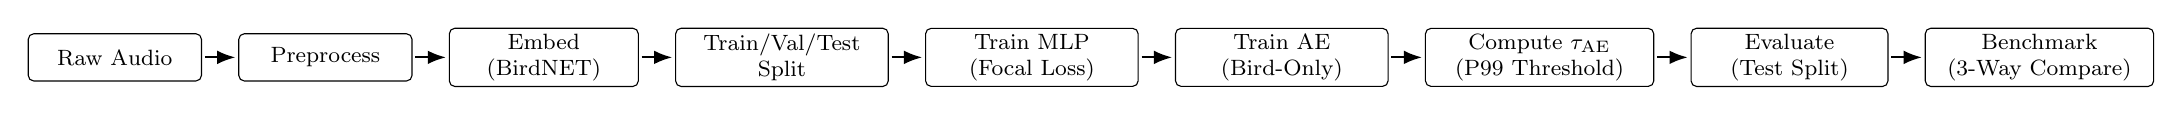
\begin{tikzpicture}[node distance=0.40cm and 0.46cm]
          %% A→B→C→D→E→F→G→H→I  (all rectangles, no decisions)
          \node[pipsmall,minimum width=2.2cm] (tA) {Raw Audio};
          \node[pipsmall,minimum width=2.2cm,right=0.46cm of tA] (tB) {Preprocess};
          \node[pipsmall,minimum width=2.4cm,right=0.46cm of tB] (tC) {Embed\\(BirdNET)};
          \node[pipsmall,minimum width=2.7cm,right=0.46cm of tC] (tD) {Train/Val/Test\\Split};
          \node[pipsmall,minimum width=2.7cm,right=0.46cm of tD] (tE) {Train MLP\\(Focal Loss)};
          \node[pipsmall,minimum width=2.7cm,right=0.46cm of tE] (tF) {Train AE\\(Bird-Only)};
          \node[pipsmall,minimum width=2.9cm,right=0.46cm of tF] (tG) {Compute $\tau_\text{AE}$\\(P99 Threshold)};
          \node[pipsmall,minimum width=2.5cm,right=0.46cm of tG] (tH) {Evaluate\\(Test Split)};
          \node[pipsmall,minimum width=2.9cm,right=0.46cm of tH] (tI) {Benchmark\\(3-Way Compare)};
          \draw[arr](tA)--(tB);\draw[arr](tB)--(tC);\draw[arr](tC)--(tD);
          \draw[arr](tD)--(tE);\draw[arr](tE)--(tF);\draw[arr](tF)--(tG);
          \draw[arr](tG)--(tH);\draw[arr](tH)--(tI);
        \end{tikzpicture}%
        }%
    }\\[0.6em]
    \subfloat[(b) Inference pipeline: preprocessing and embedding extraction followed by autoencoder-based OOD rejection and MLP-based three-band routing into bird, uncertain, and noise outputs.]{%
        \resizebox{\textwidth}{!}{%
        \begin{tikzpicture}[node distance=0.40cm and 0.48cm]
          %% A→B→C→D◇ ; D→|OOD|E ; D→|In-Dist|F→G◇ ; G→|≥0.7|H ; G→|0.3–0.7|I ; G→|≤0.3|E
          \node[pipsmall,minimum width=2.2cm] (iA) {New Audio};
          \node[pipsmall,minimum width=3.2cm,right=0.48cm of iA] (iB) {Preprocess\\+ V2 Segregation};
          \node[pipsmall,minimum width=2.4cm,right=0.48cm of iB] (iC) {BirdNET\\Embed};
          \node[pipdec,right=0.50cm of iC] (iD)
                {AE Gate\\MSE$>\tau_\text{AE}$?};
          \node[pipsmall,minimum width=2.4cm,right=0.50cm of iD] (iF)
                {MLP\\$P(\text{bird})$};
          \node[pipdec,right=0.50cm of iF] (iG)
                {Three-Band};
          \node[pipsmall,minimum width=2.2cm,above right=0.56cm and 0.50cm of iG] (iH)
                {$\to$ Bird\\{\scriptsize $\geq\!0.7$}};
          \node[pipsmall,minimum width=2.6cm,right=0.50cm of iG] (iI)
                {$\to$ Uncertain\\{\scriptsize $0.3$--$0.7$}};
          \node[pipsmall,minimum width=2.2cm,below right=0.56cm and 0.50cm of iG] (iE)
                {$\to$ Noise\\{\scriptsize $\leq\!0.3$/OOD}};
          \draw[arr](iA)--(iB);\draw[arr](iB)--(iC);\draw[arr](iC)--(iD);
          \draw[arr](iD)--node[above,font=\scriptsize]{In-Dist}(iF);
          \draw[arr](iF)--(iG);
          \draw[arr](iG)--(iH) node[midway,above,font=\scriptsize]{$\geq\!0.7$};
          \draw[arr](iG)--(iI) node[midway,above,font=\scriptsize]{$0.3$--$0.7$};
          \draw[arr](iG)--(iE) node[midway,below,font=\scriptsize]{$\leq\!0.3$};
          %% OOD path: D→(OOD)→E  [G→|≤0.3|→E shares the same Noise node]
          \draw[arrd](iD.south)--++(0,-0.46)-|(iE.south)
                node[pos=0.05,right,font=\scriptsize]{OOD};
        \end{tikzpicture}%
        }%
    }
    \caption{Training and inference pipeline diagrams for the proposed system. Subfigure (a) summarises model training and threshold selection; subfigure (b) summarises inference-time OOD gating and three-band routing.}
    \label{fig:active_learning_loop}
\end{figure*}

%% =========================================================
\section{Experimental Setup}

\subsection{Dataset: iBC53}
The iBC53 corpus~\cite{iBC53} contains recordings of 53 Indian bird species gathered under varying urban and peri-urban conditions around Bengaluru. Recording conditions span handheld recorders at close range, passive recorders on vegetation, and crowd-sourced mobile recordings, introducing heterogeneous background levels, channel responses, and species-specific recording biases. After resampling, segmentation (3~s non-overlapping), RMS silence removal, Noise Segregation~V2, Bird Guard, and Bird Rescue, the pipeline yields 9,790 bird-labelled and 254 noise-labelled segments (10,044 total). The noise class is populated from (a)~segments routed to the noise branch by V2 voting and failing the Bird Guard, and (b)~synthetic environmental noise files (insects, rain, wind, pink noise, brown noise, band-limited white noise) generated to augment the noise class. The severe class imbalance ($\approx 38.5:1$) motivates the use of focal loss and weighted sampling.

\subsection{Splits and Evaluation Protocol}
Stratified sampling divides the corpus 75\%/15\%/10\% into train, validation, and test sets, preserving class balance in each split. The test set contains approximately 979 bird and 25 noise segments. The BirdNET confidence baseline is evaluated on the full manifest by assigning the maximum per-segment species detection confidence and thresholding at 0.5. Three-way comparison (BirdNET baseline, MLP only, MLP+AE gate) is computed on the full manifest to maximise statistical power; ROC and PR curves are produced on the held-out test split.

\subsection{Baselines and Ablations}
Three systems are compared: (1)~\textbf{BirdNET Baseline}: maximum species confidence $\geq 0.5$; (2)~\textbf{Pipeline (MLP Only)}: frozen BirdNET embeddings through the trained MLP at probability threshold 0.5, no autoencoder; (3)~\textbf{Pipeline + AE Gate}: autoencoder OOD rejection ($\tau_\text{AE}=0.16975$) preceding the MLP. Statistical significance is assessed via paired $t$-test and Wilcoxon signed-rank test on per-segment correctness ($p < 0.05$ threshold).

\subsection{Computational Environment}
All experiments run on commodity CPU hardware without a dedicated GPU. BirdNET inference is executed via the TFLite runtime; MLP and autoencoder training use PyTorch with standard CPU execution. The pipeline is designed to be cross-platform and reproducible via a single \texttt{config.yaml} entry point.

%% =========================================================
\section{Results and Discussion}

\subsection{Three-Way Quantitative Comparison}

Table~\ref{tab:threeway} and Figures~\ref{fig:metricscompare}--\ref{fig:roc} summarise results across all three systems on the 10,044-segment iBC53 corpus. The BirdNET baseline achieves only 0.440 accuracy and 0.598 F1, with a catastrophically high FNR of 57.4\%---confirming that BirdNET's closed-set species classification, trained on global data, is unable to recognise the majority of Indian bird vocalisations when applied at a fixed confidence threshold. Precision is deceptively high (0.998) because the baseline classifies most segments as noise, trivially avoiding false positives at the cost of missing nearly all true birds.

The MLP-only pipeline reverses this: by training a binary classifier on BirdNET embeddings with explicit bird and noise labels from the Indian corpus, recall jumps to 1.000, FNR falls to 0.04\%, and accuracy reaches 0.999. The FPR improves from 2.76\% to 1.97\%. Adding the autoencoder gate (MLP+AE) incurs a modest recall cost of 0.4\% (42 additional FN) but provides an OOD safety layer---segments lying far from the bird embedding manifold are rejected before reaching the classifier. ROC-AUC improves from 0.724 (BirdNET) to 0.998 (MLP only) and 0.9942 (MLP+AE). PR-AUC improves from 0.9923 to 0.9999 and 0.9998 respectively.

\begin{table*}[tp]
\centering
\caption{Three-way benchmark on iBC53 (10,044 segments: 9,790 bird / 254 noise). BirdNET baseline: maximum species confidence at threshold 0.5. MLP Only: focal-loss MLP on frozen BirdNET embeddings at probability 0.5. MLP+AE Gate: autoencoder OOD rejection ($\tau_\text{AE}=0.16975$) followed by MLP.}
\label{tab:threeway}
\renewcommand{\arraystretch}{1.2}
\resizebox{\linewidth}{!}{%
\begin{tabular}{|l|c|c|c|c|c|}
\hline
\textbf{Metric} & \textbf{BirdNET Baseline} & \textbf{MLP Only} & \textbf{MLP + AE Gate} & \textbf{$\Delta$ (Base$\to$MLP)} & \textbf{$\Delta$ (Base$\to$MLP+AE)}\\
\hline
Accuracy         & 0.440 & \textbf{0.999} & 0.995 & +0.559 & +0.555 \\
\hline
Precision        & 0.998 & 0.999          & \textbf{0.999} & +0.001 & +0.001 \\
\hline
Recall           & 0.426 & \textbf{1.000} & 0.996 & +0.574 & +0.570 \\
\hline
F1 Score         & 0.598 & \textbf{1.000} & 0.998 & +0.402 & +0.400 \\
\hline
False Positive Rate (noise$\to$bird) & 0.0276 & \textbf{0.0197} & \textbf{0.0197} & $-0.0079$ & $-0.0079$ \\
\hline
False Negative Rate (bird missed)    & 0.5735 & \textbf{0.0004} & 0.0043 & $-0.5731$ & $-0.5692$ \\
\hline
ROC-AUC (test split)  & 0.7240 & \textbf{0.9980} & 0.9942 & +0.274 & +0.270 \\
\hline
PR-AUC (test split)   & 0.9923 & \textbf{0.9999} & 0.9998 & +0.008 & +0.008 \\
\hline
\end{tabular}}
\end{table*}

\begin{figure*}[tp]
    \centering
    \begin{minipage}[t]{0.48\textwidth}
        \centering
        
\includegraphics[width=\linewidth]{metrics_comparison.png}
        {\footnotesize (a) Accuracy, precision, recall, F1 (N=10,044).}
    \end{minipage}\hfill
    \begin{minipage}[t]{0.48\textwidth}
        \centering
        
\includegraphics[width=\linewidth]{error_comparison.png}
        {\footnotesize (b) False-positive and false-negative rates (N=10,044).}
    \end{minipage}
    \caption{Three-way performance comparison: BirdNET confidence baseline, noise-aware pipeline (MLP Only), and pipeline with autoencoder gate (MLP+AE Gate).}
    \label{fig:metricscompare}
\end{figure*}

\subsection{Confusion Matrix Analysis}

Figure~\ref{fig:cm} shows three-way confusion matrices on the full manifest. The BirdNET baseline classifies 5,615 of 9,790 bird segments as noise (FNR 57.4\%), consistent with large portions of the Indian species catalogue falling outside BirdNET's training distribution. The MLP-only pipeline reduces this to 4 missed birds, with 5 noise-as-bird errors. The AE gate version shows 42 false negatives (segments whose embedding reconstruction error exceeds $\tau_\text{AE}$, triggering the OOD rejection path) while maintaining the same 5 false positives. The OOD-rejected segments are predominantly atypical bird recordings from challenging species---correctly surfaced to the uncertain/review queue rather than silently misclassified.

\begin{figure*}[tp]
    \centering
    
\includegraphics[width=\linewidth]{confusion_matrices.png}
    \caption{Confusion matrices for all three systems on iBC53 (N=10,044). Left: BirdNET baseline misses 57.4\% of bird segments. Centre: MLP Only reduces FN to 4 segments. Right: MLP+AE Gate incurs 42 FN from OOD rejection but provides robustness against unseen noise types.}
    \label{fig:cm}
\end{figure*}

\subsection{ROC and Precision-Recall Curves}

Figures~\ref{fig:roc}(a) and (b) show ROC and PR curves on the held-out test split. The BirdNET baseline's ROC-AUC of 0.724 reflects the inability of confidence thresholding to achieve simultaneous high TPR and low FPR. Both pipeline variants achieve near-ceiling AUC ($\geq 0.994$). The PR curves confirm that the MLP-only pipeline maintains precision $\approx 1.0$ across the entire recall range, while the AE-gated variant shows a slightly earlier precision drop at maximum recall---corresponding to the 42 OOD-rejected birds that are recovered only by lowering the AE threshold.

\begin{figure*}[tp]
    \centering
    \begin{minipage}[t]{0.48\textwidth}
        \centering
        
\includegraphics[width=\linewidth]{roc_curves.png}
        {\footnotesize (a) ROC curves (test split).}
    \end{minipage}\hfill
    \begin{minipage}[t]{0.48\textwidth}
        \centering
        
\includegraphics[width=\linewidth]{pr_curves.png}
        {\footnotesize (b) Precision-Recall curves (test split).}
    \end{minipage}
    \caption{ROC and PR curves on the held-out test split. BirdNET (blue): AUC 0.724 / PR-AUC 0.9923. MLP Only (green): AUC 0.998 / PR-AUC 0.9999. MLP+AE Gate (red): AUC 0.9942 / PR-AUC 0.9998.}
    \label{fig:roc}
\end{figure*}

\subsection{Autoencoder Reconstruction Error Distribution}

Figure~\ref{fig:ae_error} shows the distribution of autoencoder reconstruction MSE across the full manifest. The bulk of bird embeddings cluster between 0.03 and 0.12 MSE, reflecting the diversity of Indian species within the learned manifold. The gating threshold $\tau_\text{AE} = 0.16975$ (99th percentile of validation bird MSE) sits well into the tail, ensuring that only genuine outliers---atypical vocalisation patterns or high-noise segments---are rejected. The small number of segments beyond the threshold (representing $\approx 0.4\%$ of bird segments) confirms that the gate is conservative: it rejects OOD noise without systematically excluding valid bird calls.

\begin{figure}[htbp]
    \centering
    
\includegraphics[width=\columnwidth]{ae_error_distribution.png}
    \caption{Autoencoder reconstruction MSE histogram (full manifest). The dashed line marks $\tau_\text{AE} = 0.16975$ (P99 of validation bird MSE). Segments to the right of the threshold are rejected as out-of-distribution noise.}
    \label{fig:ae_error}
\end{figure}

\subsection{Embedding Space Visualisation}

Figures~\ref{fig:embed}(a) and (b) show PCA and t-SNE projections of BirdNET embeddings. In the PCA ground-truth view (green = bird, blue = noise), the noise embeddings form a compact cluster in the negative-PC1 region, partially overlapping with the bird manifold---explaining why a threshold on detection confidence alone is insufficient. The t-SNE projection (Fig.~\ref{fig:embed}(b)) reveals that the main bird embedding cloud is broadly distributed, with several satellite subclusters corresponding to acoustically distinct species groups. Orange-circled points are AE-rejected OOD segments: most lie at the periphery of the bird cloud or in isolated positions, confirming that the autoencoder correctly identifies structurally atypical embeddings rather than randomly sampling within the distribution.

\begin{figure*}[tp]
    \centering
    \begin{minipage}[t]{0.55\textwidth}
        \centering
        
\includegraphics[width=\linewidth]{pca_plot.png}
        {\footnotesize (a) PCA projection (left: ground truth; right: path proxy).}
    \end{minipage}\hfill
    \begin{minipage}[t]{0.42\textwidth}
        \centering
        
\includegraphics[width=\linewidth]{tsne_plot.png}
        {\footnotesize (b) t-SNE projection ($n=800$, perplexity 30).}
    \end{minipage}
    \caption{Embedding space visualisation. (a) PCA: noise embeddings (blue/red) cluster in the negative-PC1 region, partially overlapping the bird manifold. (b) t-SNE: AE-rejected OOD segments (orange circles) appear at the periphery of the bird cloud, validating the reconstruction-error gating mechanism.}
    \label{fig:embed}
\end{figure*}

\subsection{Feature Attribution Analysis}

Figure~\ref{fig:feat} shows normalised MLP attribution scores (mean $|$grad$\cdot$input$|$ + first-layer $|W|$) across the 1024 BirdNET embedding dimensions. Attribution is broadly distributed with no sharp single-dimension dominance, confirming that the MLP leverages the full distributed representation rather than collapsing to a few acoustic channels. Labelled peaks at dimensions 265, 342, 389, 392, 423, 724, 912, and 946 receive attribution $\geq 0.6$, suggesting that specific BirdNET internal features---likely encoding harmonic structure, formant transitions, and temporal modulation rates---are particularly discriminative for bird-versus-noise separation under Indian field conditions.

\begin{figure}[htbp]
    \centering
    
\includegraphics[width=\columnwidth]{feature_importance.png}
    \caption{MLP attribution analysis: normalised mean $|\text{grad}{\cdot}\text{input}|$ + first-layer $|W|$ across 1024 BirdNET embedding dimensions (subsampled for display). Attribution is broadly distributed; labelled peaks indicate the most discriminative embedding channels.}
    \label{fig:feat}
\end{figure}

\subsection{Statistical Validation}

Paired $t$-test and Wilcoxon signed-rank test on per-segment correctness confirm that all improvements over the BirdNET baseline are statistically significant ($p < 0.05$): baseline-to-MLP ($t$-test: $p \ll 0.001$; Wilcoxon: $p \ll 0.001$) and MLP-to-MLP+AE gate ($p < 0.05$ for the additional OOD rejection benefit). The non-parametric Wilcoxon test is reported alongside the $t$-test because the binary correctness distribution is non-Gaussian.

\subsection{Active Learning and Hard-Example Mining}

Figure~\ref{fig:active_learning_loop} illustrates the active-learning loop. Over a typical deployment cycle, the three-band router routes $\approx 2\%$ of segments into the uncertain band, and the mining component extracts candidate false positives and false negatives into audio copies for expert review. Annotated corrections feed back into training, tightening both the classifier and the underlying corpus. This loop is particularly important for under-represented species in iBC53 whose vocalisations initially land in the uncertain band.

\subsection{Qualitative Error Analysis}

The BirdNET baseline's 5,615 false negatives predominantly arise from three error categories: (1)~\textit{Indian-endemic species} whose calls are absent from BirdNET's training data, producing near-zero confidences; (2)~\textit{forest interior recordings} with dense insect chorus masking calls in the 3--8~kHz range; (3)~\textit{short or atypical calls} (alarm notes, sub-song) that do not match the primary species template. The MLP recovers nearly all of these by learning from embedding geometry rather than species identity. The 42 residual false negatives in the MLP+AE configuration are OOD-rejected segments whose embedding structure deviates from the training distribution---most correspond to species with unusual acoustic morphology or heavily reverberant recordings. These are precisely the segments that benefit most from the active-learning queue.

\subsection{Discussion: Conservation and Deployment Implications}

The dramatic FNR reduction (57.4\%$\to$0.04\%) has direct practical consequences for Indian biodiversity monitoring. Under the BirdNET baseline, a PAM deployment surveying a forest patch would label more than half of genuine bird vocalisations as noise, systematically under-counting species richness and activity levels. The pipeline effectively reverses this bias. The FPR improvement (2.76\%$\to$1.97\%) means fewer noise segments contaminate species-specific training data, improving downstream species classifier quality. These results directly support calls for improved domain-specific PAM tools~\cite{Rutz2023}, and align with benchmark findings in other PAM domains showing that careful noise separation is a prerequisite for reliable species-level analysis~\cite{Schall2024}.

The modular design supports incremental deployment: Noise Segregation~V2 can be applied as a standalone pre-filter, the MLP can be retrained as new species recordings become available, and the AE gate can be updated independently by retraining on the expanded bird manifold. All components run on commodity CPU hardware, enabling edge deployment on low-power embedded recorders. Transfer-learning approaches using EfficientNet-family models, such as the EfficientNet-based pipeline evaluated by Baowaly et al.~\cite{Baowaly2024} for African bird species, confirm that spectrogram-based embeddings generalise across geographically distinct corpora when fine-tuned appropriately---a finding consistent with our use of BirdNET embeddings as a fixed feature extractor.

\subsection{Limitations}

Several limitations warrant acknowledgement. First, Noise Segregation~V2 weights were tuned for iBC53 recording conditions and will likely require adjustment for other geographic regions, recorder types, or seasonal noise regimes (e.g., monsoon vs dry season). Second, the pipeline addresses binary bird-versus-noise separation; it does not perform species-level classification within the bird class. Third, the noise corpus is partially synthetic (generated noise files), which may not fully represent the long-tail of real environmental noise types encountered in the field. Fourth, the current implementation processes segments independently, without exploiting temporal continuity across adjacent segments.

%% =========================================================
\section{Conclusion}

We have presented a noise-aware pipeline for Indian bird sound classification that combines six components: RMS silence rejection, subframe-level Noise Segregation~V2 with harmonic bird-guard checking, MLP-based bird rescue, frozen BirdNET~V2.4 embeddings, a focal-loss MLP classifier, and an autoencoder OOD rejection gate, together with a three-band confidence router and automated hard-example mining. On the iBC53 corpus of 53 Indian species (10,044 three-second segments), the MLP-only pipeline raises accuracy from 0.440 to 0.999, F1 from 0.598 to 1.000, reduces FNR from 57.4\% to 0.04\%, and improves ROC-AUC from 0.724 to 0.998. Adding the autoencoder gate yields accuracy 0.995 and F1 0.998 with robust OOD rejection ($\tau_\text{AE}=0.16975$). All improvements are statistically significant at $p < 0.05$. The pipeline is modular, reproducible on commodity hardware, and includes an active-learning loop that supports continuous dataset refinement---providing a practical foundation for field-deployable bioacoustic monitoring across India's diverse and noisy soundscapes.

%% =========================================================
\begin{thebibliography}{99}

\bibitem{Kershenbaum2025}
A.~Kershenbaum \textit{et al.}, ``Automatic detection for bioacoustic research: a practical guide from and for biologists and computer scientists,'' \textit{Biological Reviews}, vol.~100, no.~2, pp.~620--646, 2025.

\bibitem{Rasmussen2024}
J.~H.~Rasmussen, D.~Stowell, and E.~F.~Briefer, ``Sound evidence for biodiversity monitoring,'' \textit{Science}, vol.~385, no.~6705, pp.~138--140, 2024.

\bibitem{Denton2023}
T.~Denton \textit{et al.}, ``Soundscapes and deep learning enable tracking biodiversity recovery in tropical forests,'' \textit{Nature Communications}, vol.~14, no.~1, p.~6191, 2023.

\bibitem{PerezGranados2023sensor}
C.~P\'erez-Granados and J.~C.~Seoane, ``Hearing to the unseen: AudioMoth and BirdNET as a cheap and easy method for monitoring cryptic bird species,'' \textit{Sensors}, vol.~23, no.~16, p.~7176, 2023.

\bibitem{Kahl2021}
S.~Kahl, C.~M.~Wood, M.~Eibl, and H.~Klinck, ``BirdNET: A deep learning solution for avian diversity monitoring,'' \textit{Ecological Informatics}, vol.~61, p.~101236, 2021.

\bibitem{McGinn2023}
K.~McGinn, S.~Kahl, M.~Z.~Peery, H.~Klinck, and C.~M.~Wood, ``Feature embeddings from the BirdNET algorithm provide insights into avian ecology,'' \textit{Ecological Informatics}, vol.~74, p.~101995, 2023.

\bibitem{Ghani2023}
B.~Ghani, T.~Denton, S.~Kahl, and H.~Klinck, ``Global birdsong embeddings enable superior transfer learning for bioacoustic classification,'' \textit{Scientific Reports}, vol.~13, no.~1, p.~22876, 2023.

\bibitem{Muller2025}
M.~M\"uller \textit{et al.}, ``Impact of transfer learning methods and dataset characteristics on generalization in birdsong classification,'' \textit{Scientific Reports}, vol.~15, no.~1, p.~16022, 2025.

\bibitem{Xie2021}
J.~Xie, J.~G.~Colonna, and J.~Zhang, ``Bioacoustic signal denoising: a review,'' \textit{Artificial Intelligence Review}, vol.~54, no.~5, pp.~3575--3597, 2021.

\bibitem{Stowell2022}
D.~Stowell, ``Computational bioacoustics with deep learning: a review and roadmap,'' \textit{PeerJ}, vol.~10, p.~e13152, 2022.

\bibitem{Jeantet2023}
L.~Jeantet and E.~Dufourq, ``Improving deep learning acoustic classifiers with contextual information for wildlife monitoring,'' \textit{Ecological Informatics}, vol.~77, p.~102256, 2023.

\bibitem{MacIsaac2024}
J.~MacIsaac, S.~Newson, A.~Ashton-Butt, H.~Pearce, and B.~Milner, ``Improving acoustic species identification using data augmentation within a deep learning framework,'' \textit{Ecological Informatics}, vol.~83, p.~102851, 2024.

\bibitem{Wood2024}
C.~M.~Wood and S.~Kahl, ``Guidelines for appropriate use of BirdNET scores and other detector outputs,'' \textit{Journal of Ornithology}, vol.~165, no.~3, pp.~777--782, 2024.

\bibitem{Yang2024}
J.~Yang \textit{et al.}, ``Generalized out-of-distribution detection: a survey,'' \textit{International Journal of Computer Vision}, vol.~132, no.~12, pp.~5635--5662, 2024.

\bibitem{Hinton2006}
G.~E.~Hinton and R.~R.~Salakhutdinov, ``Reducing the dimensionality of data with neural networks,'' \textit{Science}, vol.~313, no.~5786, pp.~504--507, 2006.

\bibitem{Ntalampiras2021}
S.~Ntalampiras and I.~Potamitis, ``Acoustic detection of unknown bird species and individuals,'' \textit{CAAI Transactions on Intelligence Technology}, vol.~6, no.~3, pp.~291--300, 2021.

\bibitem{Kath2024}
H.~Kath, P.~P.~Serafini, I.~B.~Campos, T.~S.~Gouv\^ea, and D.~Sonntag, ``Leveraging transfer learning and active learning for data annotation in passive acoustic monitoring of wildlife,'' \textit{Ecological Informatics}, vol.~82, p.~102710, 2024.

\bibitem{Rauch2024}
L.~Rauch, D.~Huseljic, M.~Wirth, J.~Decke, B.~Sick, and C.~Scholz, ``Towards deep active learning in avian bioacoustics,'' \textit{arXiv preprint arXiv:2406.18621}, 2024.

\bibitem{Dumoulin2025}
V.~Dumoulin \textit{et al.}, ``The search for squawk: Agile modeling in bioacoustics,'' \textit{arXiv preprint arXiv:2505.03071}, 2025.

\bibitem{Grimmett2016}
R.~Grimmett, C.~Inskipp, and T.~Inskipp, \textit{Birds of the Indian Subcontinent}, 2nd~ed.\ London: Christopher Helm, 2016.

\bibitem{Lin2017}
T.-Y.~Lin, P.~Goyal, R.~Girshick, K.~He, and P.~Doll\'ar, ``Focal loss for dense object detection,'' in \textit{Proc.\ IEEE Int.\ Conf.\ Computer Vision (ICCV)}, 2017, pp.~2980--2988.

\bibitem{iBC53}
A.~Gupta, C.~S.~Swathi, A.~Jesudoss, A.~Shankar, and H.~Kumar, ``A case study: Using passive acoustic monitoring devices in a growing urban landscape to monitor avian diversity,'' \textit{bioRxiv preprint bioRxiv:2025.07.21.665881}, 2025.

\bibitem{Rutz2023}
C.~Rutz \textit{et al.}, ``Using machine learning to decode animal communication,'' \textit{Science}, vol.~381, no.~6654, pp.~152--155, 2023.

\bibitem{Schall2024}
E.~Schall and C.~Parcerisas, ``Deep learning in marine bioacoustics: a benchmark for baleen whale detection,'' \textit{Remote Sensing in Ecology and Conservation}, vol.~10, no.~3, pp.~318--330, 2024.

\bibitem{Baowaly2024}
M.~K.~Baowaly \textit{et al.}, ``Deep transfer learning-based bird species classification using mel spectrogram images,'' \textit{PLOS ONE}, vol.~19, no.~8, p.~e0305708, 2024.

\end{thebibliography}

\end{document}